\documentclass[letterpaper]{article}
\usepackage[spanish,es-tabla]{babel}
\usepackage{indentfirst}
\usepackage{float}
\usepackage[utf8]{inputenc}
\usepackage{graphicx}

\begin{document}

\section{Ejercicio 3}

\begin{equation}
    x[n]=\delta[n]+\delta[n-1]+\delta[n-2]+\delta[n-3]
\end{equation}

\subsection{Calculo de la DTFT y la DFT}

Utilizando la definción de la DTFT:
\begin{equation}
    X(e^{j\omega})=\sum_{n=-\infty}^{\infty}x[n]e^{-j\omega n}
\end{equation}
Donde:
\begin{equation}
    \label{omega}
    \omega=2\pi f
\end{equation}
Llegamos a:
\begin{equation}
    \label{DTFT.R}
    X(e^{j\omega})=1+e^{-j\omega}+e^{-2j\omega}+e^{-3j\omega}
\end{equation}
Para el cálculo de la DFT utilizamos la ecuación:
\begin{equation}
    X[k]=\sum_{n=0}^{N-1}x[n]e^{-j\omega_k n}
\end{equation}
Donde:
\begin{equation}
    \label{omega.k}
    \omega_k=\frac{2\pi k}{N}
\end{equation}
Obteniendo:
\begin{equation}
    \label{DFT.R}
    X[k]=1+e^{\frac{-j2\pi k }{4}}+e^{\frac{-j4\pi k}{4}}+e^{\frac{-j6\pi k}{4}}
\end{equation}
Al comparar los resultados, ecuación \ref{DTFT.R} con ecuación \ref{DFT.R}, se observa que la diferencia recae en la frecuencia. Debido a esto, en la ecuación 
\ref{DTFT.R} la frecuencia asociada es la ecuación \ref{omega} que toma valores para todo $f$ dando como resultado un espectro continuo en frecuencia. Esto es un incoveniente a la hora 
de realizar el cálculo numérico (por los infinitos valores).Por esto para la \textit{DFT} se discretiza la frecuencia angular dando como resultado la ecuación \ref{omega.k}. Se concluye que es imposible encontrar de forma exacta la \textit{DTFT} a partir de la \textit{DFT}. En otras palabras, se puede decir que 
la \textit{DFT} muestrea el espectro continuo de la \textit{DTFT}.

\subsubsection{Calculo de la DFT con distintos puntos}    
Se generaron las señales con N=3, N=4 y N=8 y con dichas señales se calculo la DFT mediante la \textit{fft} y se obtuvieron los graficos presentando en la figura \ref{fig.3b}:

\begin{figure}[htb]
\centering
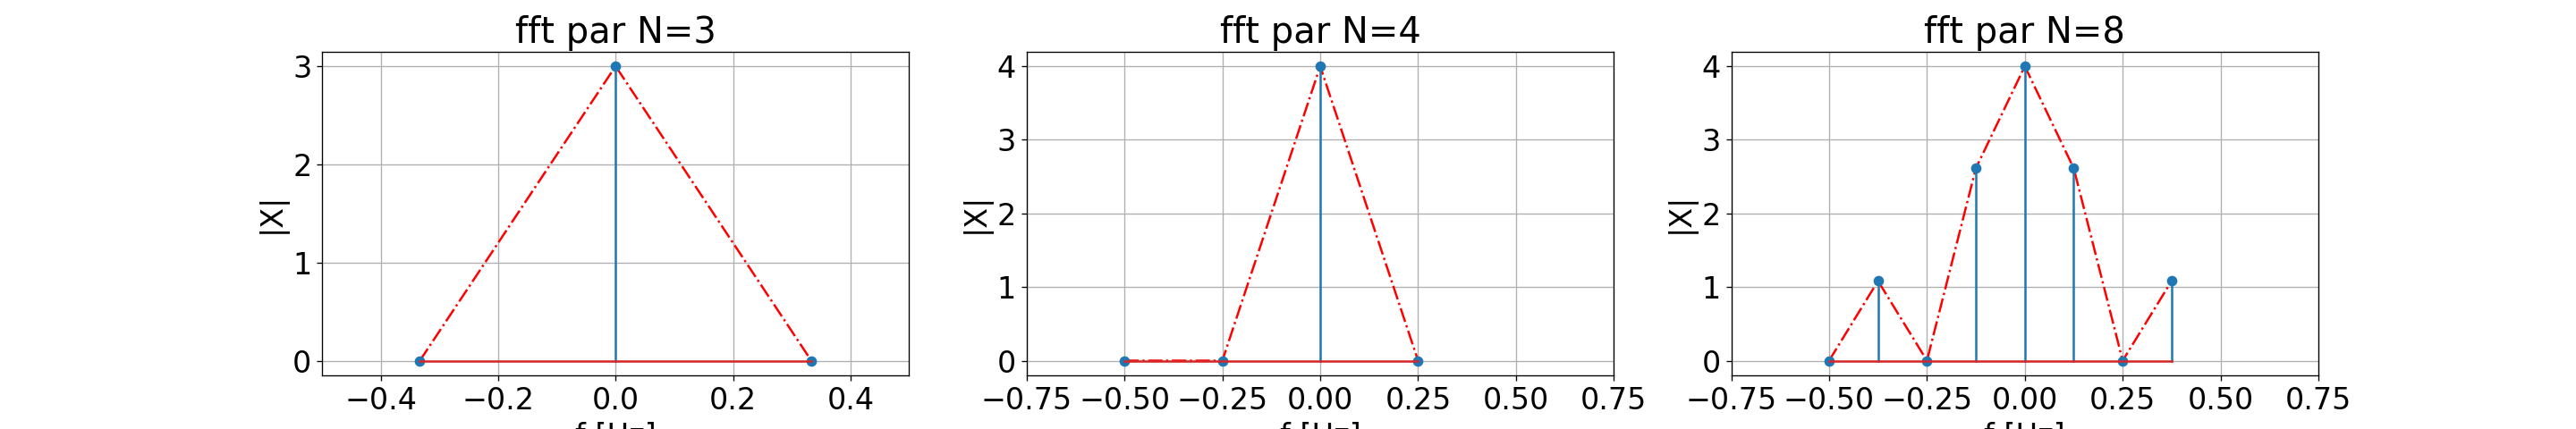
\includegraphics[width=\textwidth]{Img/punto_3_b.png}
\caption{Espectros generados con 3,4 y 8 puntos.}
\label{fig.3b}
\end{figure}

Se añadio en los graficos una señal punteada que corresponde al espectro real de la señal $x[n]$.
Se puede apreciar que los valores que toma la DFT coinciden con el valor de la envolvente en dichos puntos, por lo que seria posible aproximar la DTFT con la DFT.

\subsection{DTF con zero-padding}
Se realizo ahora nuevamente el calculo de la DFT de las señales de la seccion anterior pero ahora con el objetivo de estudiar el efecto del \textit{zero-padding}, el cual consiste en rellenar con ceros una señal hasta un numero determinado de puntos. Se tomaron las señales anteriores y se rellenaron con ceros hasta tener 256 puntos para luego calcular su DFT, los resultados obtenidos se muestran en la figura \ref{fig.1c}
\begin{figure}[htb]
\centering
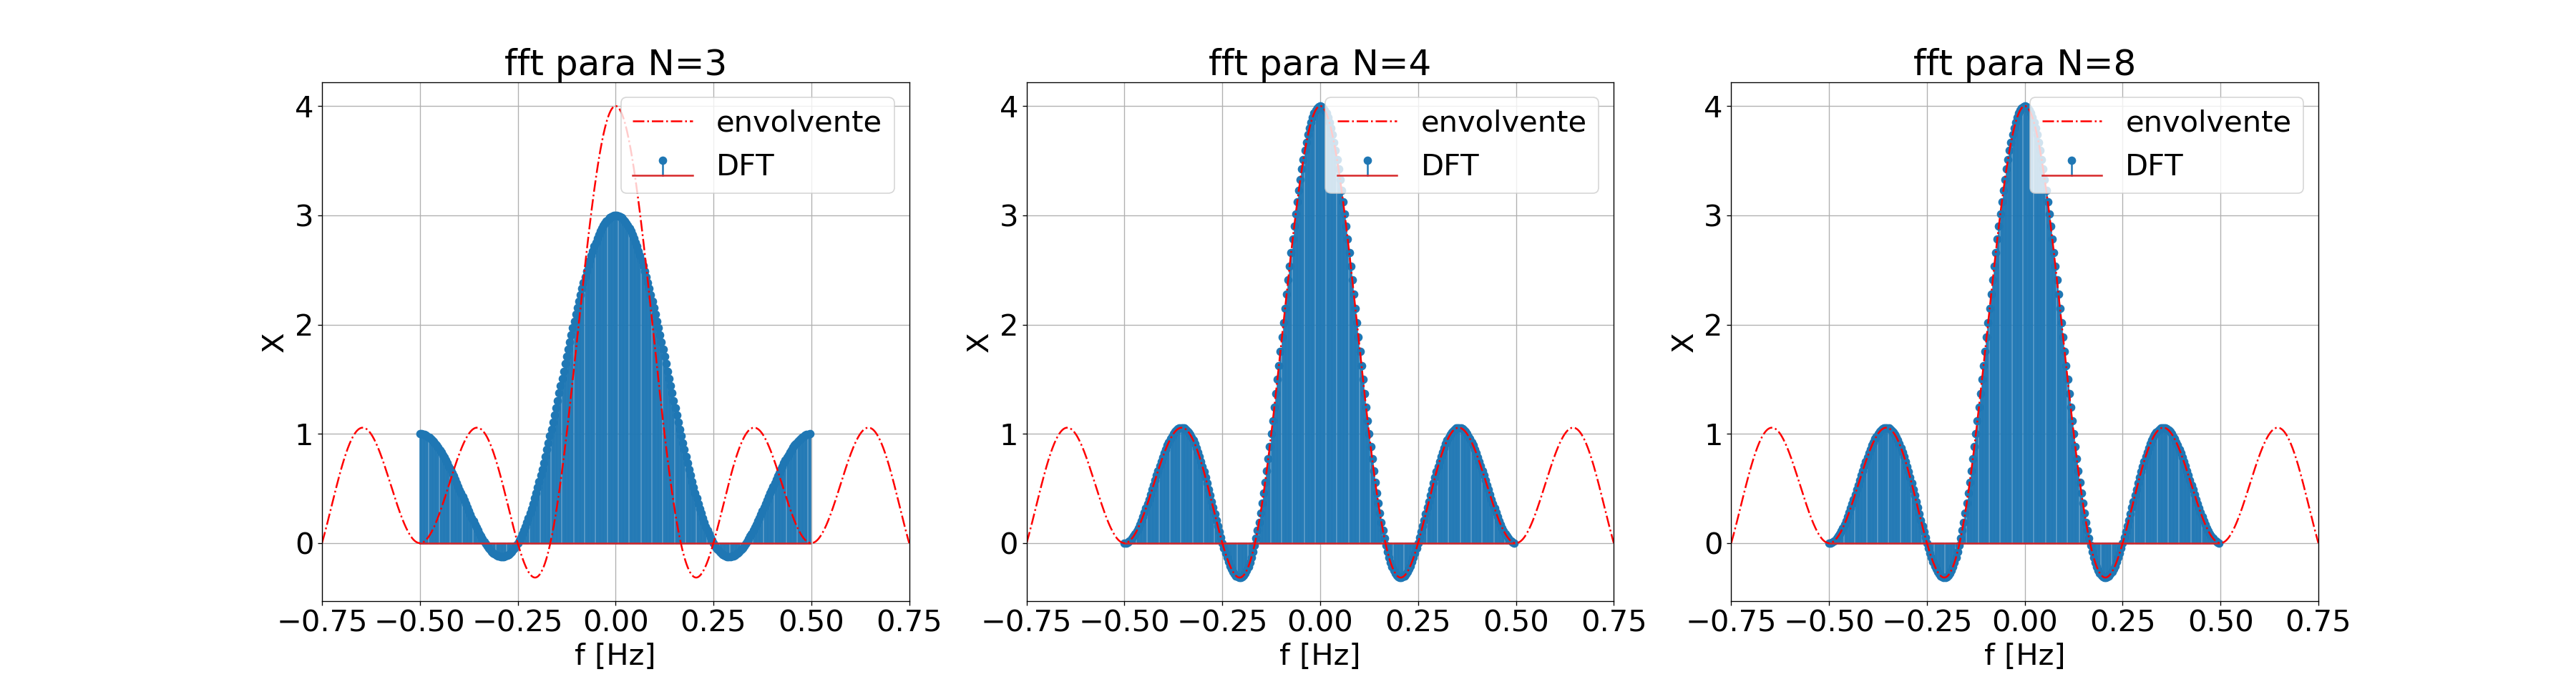
\includegraphics[width=\textwidth]{Img/punto_3_c.png}
\caption{\textit{fft} con zero-padding hasta 256 puntos para 3,4 y 8 puntos de la señal $x[n]$}
\label{fig.1c}
\end{figure}
Ahora es posible observar de mejor manera, lo comentado en el apartado anterior, como el zero-padding no agrega mas informacion al espectro sino que permite una mejor visualización del mismo, cuando se toman 3 puntos de la señal original, no se llega a tomar la señal completa si no que se recorta, por lo que el espectro si bien un aspecto similar, es mas ancho y de menor amplitud(al ser un cajon de 3 puntos y no de 4 puntos como la señal original), y para los casos de N=4 y N=8 que si se utiliza toda la informacion de la señal $x[n]$ se ve claramente que los valores de la DFT corresponden a muestras de la DTFT.


\subsection{Calculo exacto de la DTFT}

    Para obtener la DTFT a partir de la \textit{fft}, la cual se puede asociar a un muestreo del espectro
    de la DTFT, mediante la siguiente relacion 

    \begin{equation}
        X[k]=X_{DTFT}\left(  \frac{2 \pi}{N} k \right)
    \end{equation}

    Donde $N$ es el numero de puntos que se utilizan para calcular la DFT.

    El calculo de la DTFT mediante el algoritmo de la \textit{fft} nunca sera exacto. Debido a que la DTFT es continua en frecuencia 
    mientras que la la DFT no. Pero los valores obtenido de la \textit{fft}, pueden ser considerados como muestras del espectro siempre que se 
    cumpla que 

    \begin{enumerate}
        \item Señal sea de duracion finita ($L$).
        \item Utilizar al menos $L$ puntos.
    \end{enumerate}
    


   
   \subsection{codigo para la obtencion de la DTFT}
Resultado teórico de cada una de las ecuaciones: 

\subsubsection*{i)}
\begin{equation}
x_{1}[n] = \left\{ 
    \begin{array}{ll} 
    n & \mathrm{si\ } 0\leq n \leq 4 \\
    10-n & \mathrm{si\ } 5\leq n \leq 10 \\
    0 & \mathrm{sino\ } \\
    \end{array} 
    \right.
\end{equation}
Por tabla se llega al resultado:
\begin{equation}
X_{1}(e^{j \omega})=25 sinc^{2}\left(\frac{5 \omega}{2 \pi}\right) e^{- j \omega} 
\end{equation}

\subsubsection*{ii)}
\begin{equation} 
    x_{2}[n] = \left\{ 
    \begin{array}{ll} 
    1 & \mathrm{si\ } -2\leq n \leq +2, \\
    0 & \mathrm{sino\ } \\
    \end{array} 
    \right.
\end{equation}

Mediante el uso de tablas de transformada se llego a que el espectro esta dado por:
\begin{equation}
X_{2}(e^{j \omega})= \frac{sin(\frac{ \omega 5}{2})}{sin (\frac{\omega}{2})}
\end{equation}

\subsubsection*{iii)}
\begin{equation} 
    x_{3}[n]=(-0,5)^{n}u[n]
\end{equation}
Donde nuevamente su espectro se obtuvo por tablas, dando como resultado:
\begin{equation}
X(e^{j \omega})=\frac{1}{1+0,5 e^{j \omega}}
\end{equation}
Mediante la implementacion del codigo se calculo la DTFT y se obtuvieron las siguiente figuras:
\begin{figure}[H]
\centering
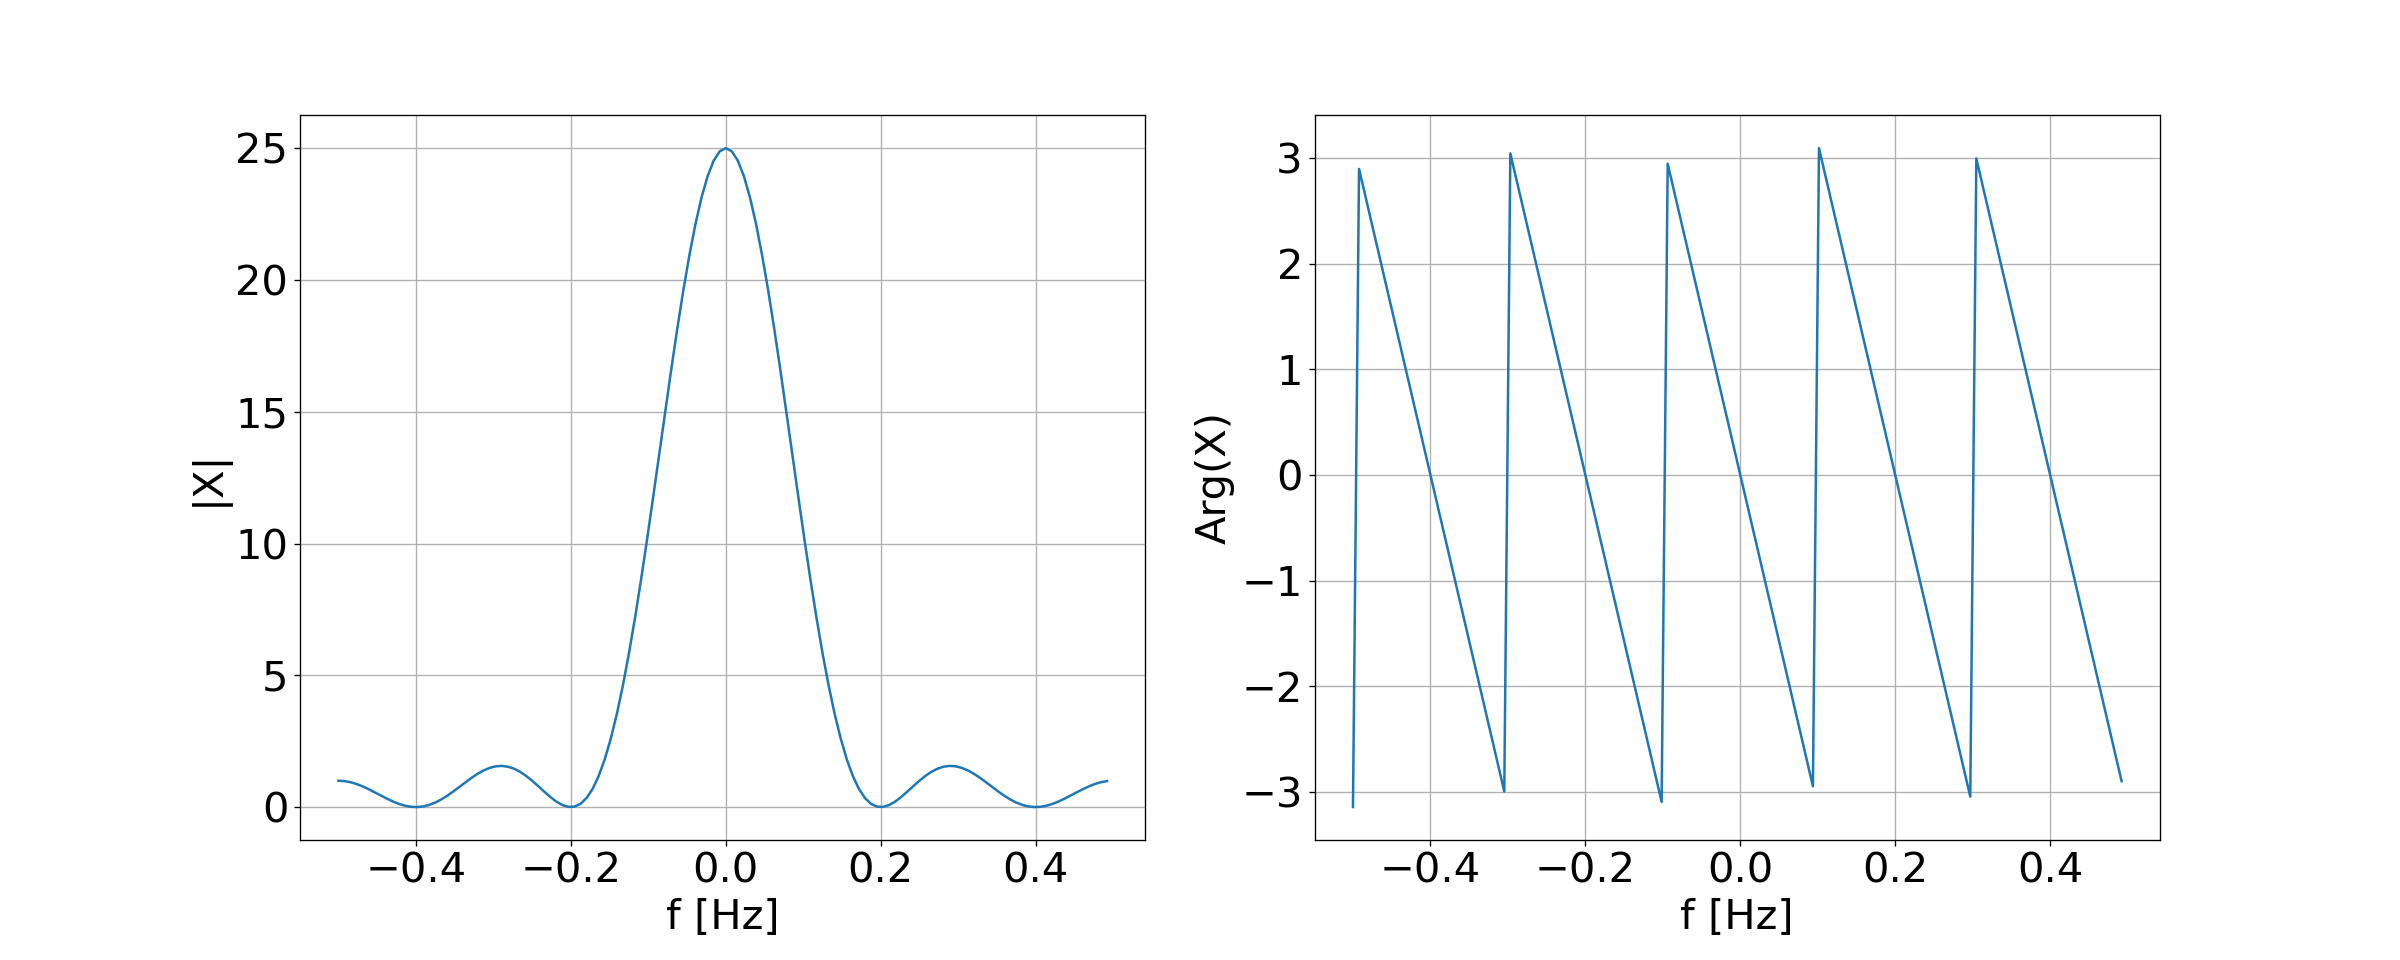
\includegraphics[width=\textwidth]{Img/punto_3_e_1.png}
\caption{Espectro de la señal $x_{1}[n]$ mediante el algoritmo.}
\label{fig.3ei}
\end{figure}

\begin{figure}[H]
\centering
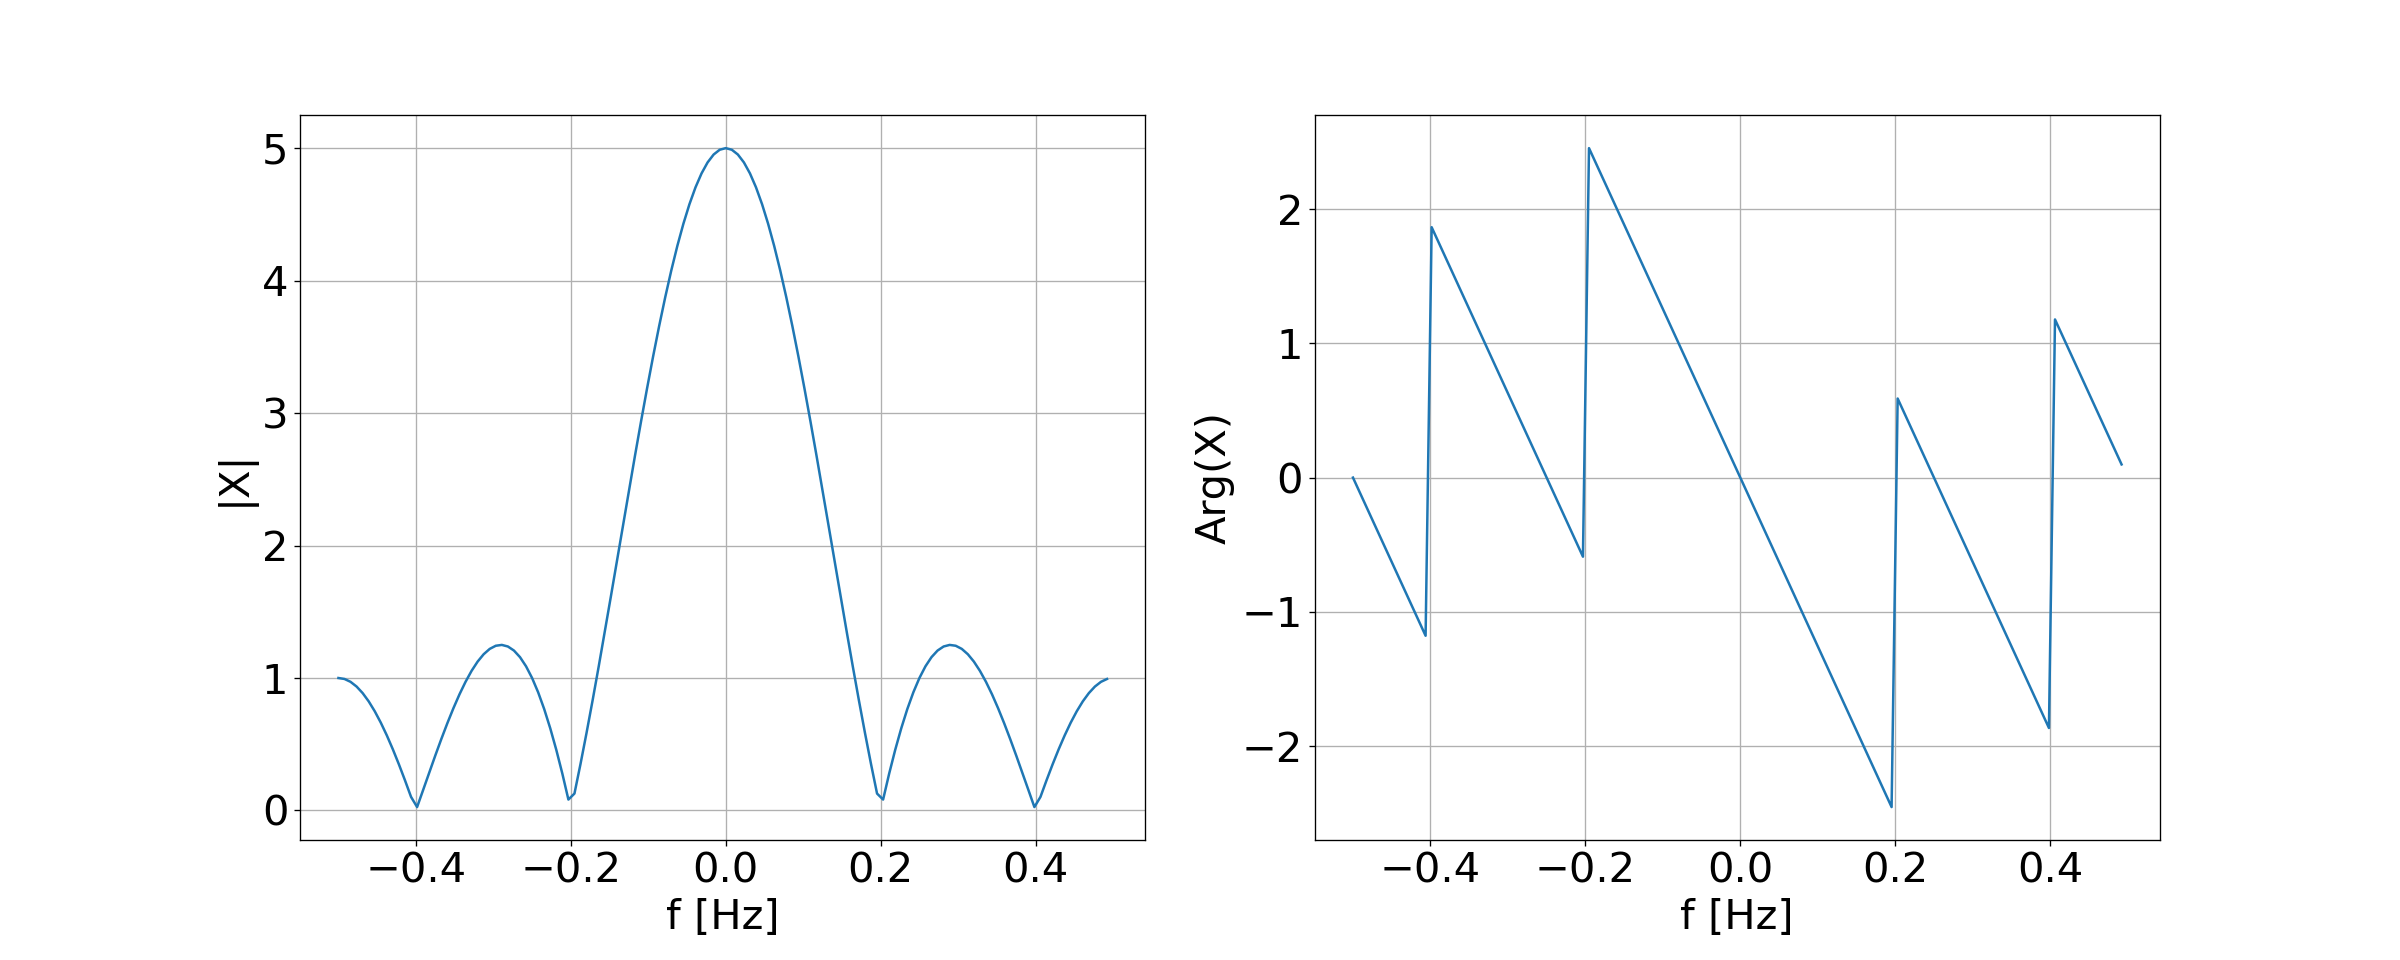
\includegraphics[width=\textwidth]{Img/punto_3_e_2.png}
\caption{Espectro de la señal $x_{2}[n]$ mediante el algoritmo.}
\label{fig.3eii}
\end{figure}

\begin{figure}[H]
\centering
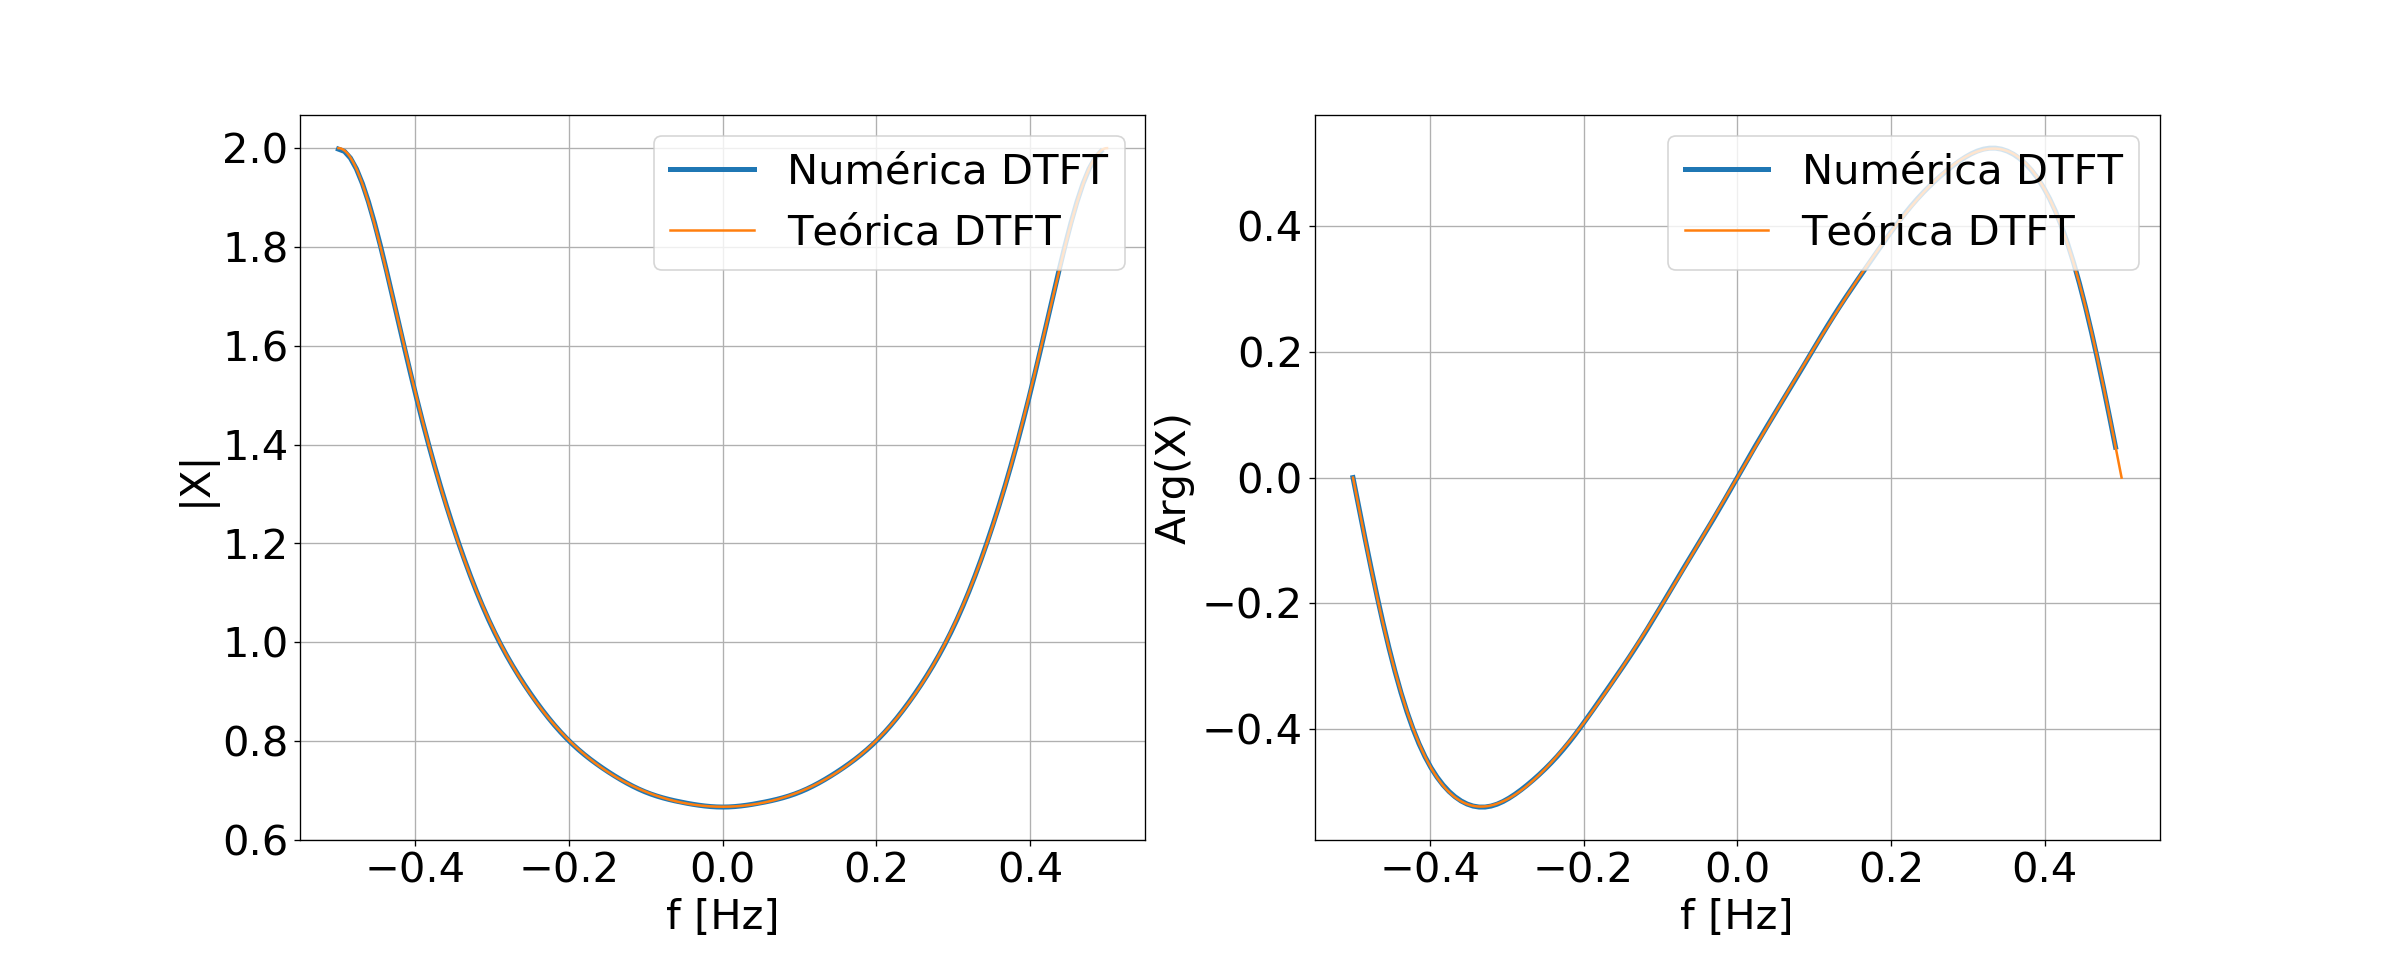
\includegraphics[width=\textwidth]{Img/punto_3_e_3.png}
\caption{Espectro de la señal $x_{3}[n]$ mediante el algoritmo.}
\label{fig.3eiii}
\end{figure}
\end{document}
Se puede apreciar que los espectros representados en las figuras \ref{fig.3ei},\ref{fig.3eii} y \ref{fig.3eiii} coinciden de manera aproximada con lo obtenido de manera teorica. 

   \end{document}